\section{Τίτλος}

\begin{figure}[h!]
    \centering
    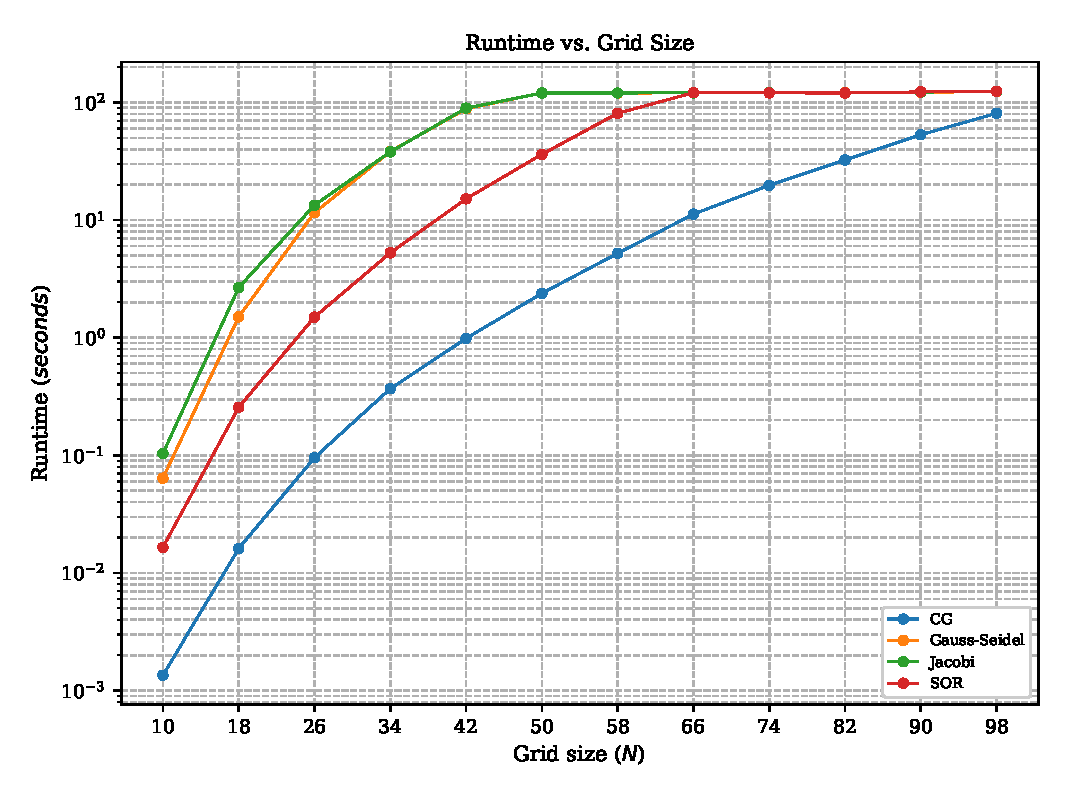
\includegraphics[width=0.80\linewidth]{doc/figures/runtime_gridsize.eps}
    \caption{Σύντομη περιγραφή}
    \label{fig:placeholder}
\end{figure}

\begin{image}
    \centering
    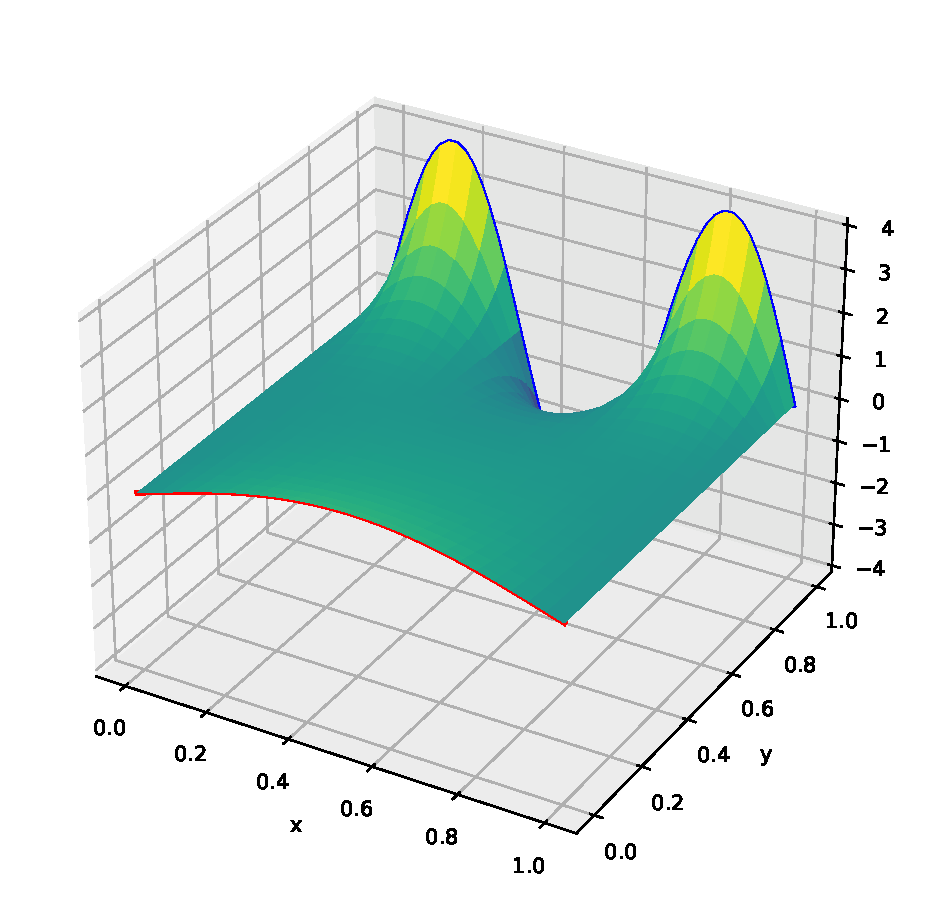
\includegraphics[width=0.70\textwidth]{doc/images/surface_plot.eps}
    \caption{Σύντομη περιγραφή}
    \label{img:example}
\end{image}


\begin{table}
    \centering
    \begin{tabular}{|c|c|c|c|c|}
    \hline
     N & \en{CG} & \en{Gauss-Seidel} & \en{Jacobi} & \en{SOR} \\
    \hline
    10 & 0.00104029 & 0.068981 & 0.107458 & 0.0152744 \\ \hline
    18 & 0.0152874 & 1.50789  & 3.02971  & 0.238877   \\  \hline
    26 & 0.0951215 & 12.5706  & 13.3289  & 1.47111    \\  \hline
    34 & 0.378859  & 37.9215  & 38.7912  & 5.46448    \\  \hline
    42 & 1.0885    & 88.8494  & 91.3744  & 15.6591    \\ \hline
    50 & 2.61074   & 178.969  & 182.915  & 37.1739    \\ \hline
    58 & 5.4616    & 338.574  & 342.548  & 81.3633    \\ \hline
    66 & 12.1681   & 578.988  & 588.112  & 156.654    \\ \hline
    74 & 21.4958   & 911.327  & 926.782  & 298.101    \\ \hline
    82 & 35.7552   & 1383.19  & 1398.03  & 540.376    \\ \hline
    90 & 56.7926   & 2000.25  & 2028.41  & 911.951    \\ \hline
    98 & 87.2408   & 2778.52  & 2843.33  & 1465.69    \\ 
    \hline
    \end{tabular}
    \caption{Σύντομη περιγραφή}
    \label{tab:computation-times}
\end{table}